% -*- Mode:TeX -*-

%% IMPORTANT: The official thesis specifications are available at:
%%            http://libraries.mit.edu/archives/thesis-specs/
%%
%%            Please verify your thesis' formatting and copyright
%%            assignment before submission.  If you notice any
%%            discrepancies between these templates and the 
%%            MIT Libraries' specs, please let us know
%%            by e-mailing thesis@mit.edu

%% The documentclass options along with the pagestyle can be used to generate
%% a technical report, a draft copy, or a regular thesis.  You may need to
%% re-specify the pagestyle after you \include  cover.tex.  For more
%% information, see the first few lines of mitthesis.cls. 

%\documentclass[12pt,vi,twoside]{mitthesis}
%%
%%  If you want your thesis copyright to you instead of MIT, use the
%%  ``vi'' option, as above.
%%
%\documentclass[12pt,twoside,leftblank]{mitthesis}
%%
%% If you want blank pages before new chapters to be labelled ``This
%% Page Intentionally Left Blank'', use the ``leftblank'' option, as
%% above. 
\def\college{Caan Institute for Advanced Study}
\documentclass[12pt,twoside]{cuthesis}
\def\mystretch{2}	
\usepackage{lgrind}
%% These have been added at the request of the MIT Libraries, because
%% some PDF conversions mess up the ligatures.  -LB, 1/22/2014
\usepackage{cmap}
\usepackage{graphicx}
\usepackage{textcomp}
\usepackage{tikz}
\usepackage{pgfplots}
\pgfplotsset{width=10cm,compat=1.9} 
\usepackage{fancyhdr}
\usepackage{tikz-3dplot}
\usetikzlibrary{tikzmark}
\usepgfplotslibrary{external}
\usetikzlibrary{positioning}
\usepackage{amssymb}
\usepackage{amsmath}
\usepackage{amsfonts}
\graphicspath{ {images/} }
\usepackage[T1]{fontenc}
\pagestyle{plain}

%% This bit allows you to either specify only the files which you wish to
%% process, or `all' to process all files which you \include.
%% Krishna Sethuraman (1990).

%\typein [\files]{Enter file names to process, (chap1,chap2 ...), or `all' to
%process all files:}
%\def\all{all}
%\ifx\files\all \typeout{Including all files.} \else \typeout{Including only \files.} \includeonly{\files} \fi
\fancyfoot{}
\fancyhead[RO,LE]{\thepage}
\fancyhead[LO]{\leftmark}
\fancyhead[RE]{\rightmark}

\begin{document}
\include{cover}
\pagenumbering{Roman} 
% Some departments (e.g. 5) require an additional signature page.  See
% signature.tex for more information and uncomment the following line if
% applicable.
% \include{signature}
%\pagestyle{plain}
\pagestyle{fancy}
\setlength{\headheight}{15pt} 
\include{contents}
% chap1 = Intro, specific aims, scott caan
\pagenumbering{arabic} 
%% This is an example first chapter.  You should put chapter/appendix that you
%% write into a separate file, and add a line \include{yourfilename} to
%% main.tex, where `yourfilename.tex' is the name of the chapter/appendix file.
%% You can process specific files by typing their names in at the 
%% \files=
%% prompt when you run the file main.tex through LaTeX.
\chapter{Introduction}

\section{Motivations}

\begin {figure}[htbp]
\centering
\includegraphics[width=\textwidth]{scottcaan1}
\caption{Scott Caan}
\label{fig1}
\centering
\end{figure}
\subsection{Specific aim 1: Scott Caan }

        	Scott Caan, scott caan scott caan scott caan? Scott "caan" scott caan scott "caan": scott caan, scott caan scott, caan scott caan scott. Scott caan scott.
\subsection{Specific Aim 2: Scott Caan}

Scott caan scott caan scott caan. Scott "caan", scott caan scott\cite{caan1}, caan scott, caan scott.
 
\begin {figure}[htbp]
\centering
\includegraphics[scale=.5]{scottcaan2}
\caption{Scott Caan}
\label{fig2}
\centering
\end{figure}

 
\subsection {Specific aim 3: Scott Caan}

Scott caan, scott caan scott, caan\cite{caan2} "scott caan", scott caan. Scott caan; scott, caan, scott, caan scott. 

\section{Innovation}
Scott caan? Scott caan.
\begin {figure}[htbp]
\centering
\includegraphics[scale=0.5]{scottcaan3}
\caption{Scott Caan}
\label{fig3}
\centering
\end{figure}

\section{Background}

\subsection{Scott Caan}
	Scott caan scott. Scott caan scott caan scott: caan scott caan.
\subsection{Scott Caan}
	Scott caan scott? Caan scott caan scott. Caan scott caan scott, caan scott. 
\begin {figure}[htbp]
\centering
\includegraphics[scale=.5]{scottcaan4}
\caption{Scott Caan}
\label{fig4}
\centering
\end{figure}

Scott caan scott caan scott caan scott, caan scott caan.\cite{caan3} "Scott Caan", scott caan scott caan. Scott Caan.
 

\subsection{Abbreviations}
\textbf{SC} Scott Caan

% chap2 = Scott Caan
%% This is an example first chapter.  You should put chapter/appendix that you
%% write into a separate file, and add a line \include{yourfilename} to
%% main.tex, where `yourfilename.tex' is the name of the chapter/appendix file.
%% You can process specific files by typing their names in at the 
%% \files=
%% prompt when you run the file main.tex through LaTeX.
%   _____ ______      __  _____             
%  / ____|  _ \ \    / / |  __ \            
% | |    | |_) \ \  / /  | |  | | _____   __
% | |    |  _ < \ \/ /   | |  | |/ _ \ \ / /
% | |____| |_) | \  /    | |__| |  __/\ V / 
%  \_____|____/   \/     |_____/ \___| \_/  
%                                           
%                                           

\chapter{Specific Aim 1: Scott Caan}

\section{Scott Caan}

\subsection{Introduction and study design}
 Scott Caan?\cite{caan4}
\subsection{Methods}
\begin {figure}[htbp]
\centering
\includegraphics[scale=.5]{scottcaan5}
\caption{Scott Caan}
\label{fig5}
\centering
\end{figure}
Scott Caan...
\subsection{Results and discussion}


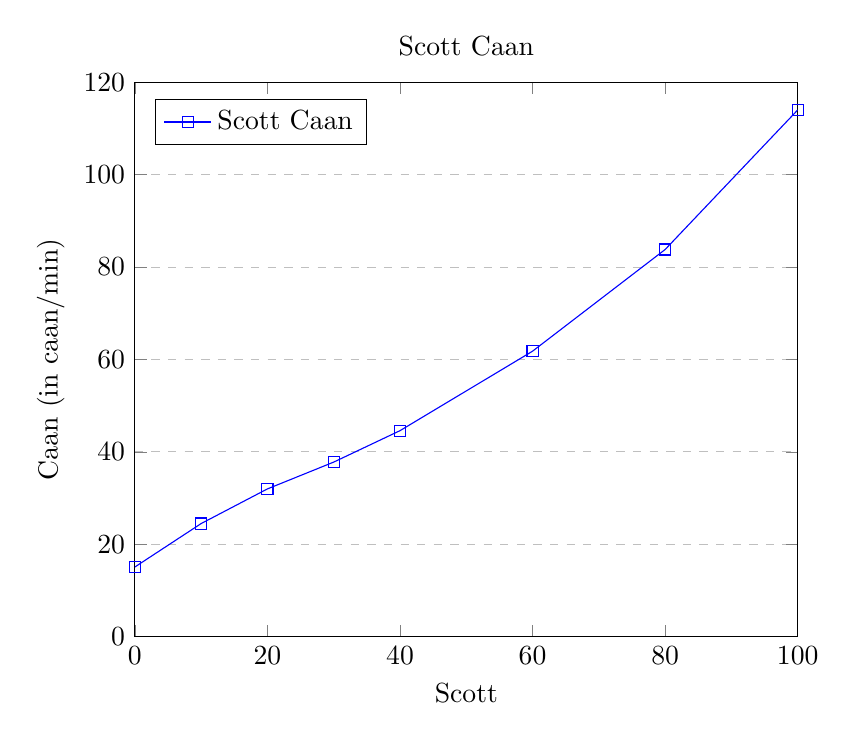
\begin{tikzpicture}
\begin{axis}[
    title={Scott Caan},
    xlabel={Scott},
    ylabel={Caan (in caan/min)},
    xmin=0, xmax=100,
    ymin=0, ymax=120,
    xtick={0,20,40,60,80,100},
    ytick={0,20,40,60,80,100,120},
    legend pos=north west,
    ymajorgrids=true,
    grid style=dashed,
]
 
\addplot[
    color=blue,
    mark=square,
    ]
    coordinates {
    (0,15.1)(10,24.5)(20,32)(30,37.8)(40,44.6)(60,61.8)(80,83.8)(100,114)
    };
    \legend{Scott Caan}
 
\end{axis}
\end{tikzpicture}



Scott Caan.
\subsection{Conclusion}
Scott Caan!\cite{caan5}
% chap3 = Scott Caan

\pagestyle{plain}
\appendix
\chapter{Appendix}
\begin{table}[]
\centering
\caption{Scott Caan}
\label{table1}
\begin{tabular}{ll}
Actor                    & Boolean \\
Scott Caan          & TRUE    \\
Greogory Peck    & FALSE  
\end{tabular}
\end{table}

\include{biblio}
\end{document}

